\documentclass[11pt,a4j,twocolumn]{jarticle}
\usepackage{csbstp}
\usepackage{amsmath}
\usepackage[dvipdfmx]{graphicx}
\usepackage{amssymb}
\usepackage{algorithm}
\usepackage{algorithmic}
\usepackage{subcaption}
\usepackage[dvipdfmx]{color}

\def\AgentSet{A}
\def\Dreq{{D_{\it req}}}
\def\En{\mathcal{E}}

\def\PausingInt{{S_{\it pause}}}
\def\PauseTimeFactor{{\gamma_{\it p}}}


\title{マルチエージェント協調巡回問題におけるエネルギー消費抑制手法の提案}
\author{松本~航平}
\studentid{1W193102}
\university{早稲田大学}
\faculty{基幹理工学部}
\department{情報理工学科}
\advisor{菅原~俊治}
\type{卒業論文}
\nendo{2022}
\hizuke{\today}

\begin{document}
\maketitle
\section{序論}
近年,ロボット技術が発達し,巡回パトロールや清掃などといった,
人間が日常的に繰り返す作業を複数の自律ロボットで代替する動きが加速している.
このような複数のロボットが協調して共通の作業を行う問題は,マルチエージェント協調巡回問題(MACPP)と呼ばれる.
MACPPでは,複数のエージェントが協力・協調することで,与えられた環境で効率的に巡回を行うことを目的とし,様々な研究がある\cite{Yoneda2013,Wu2019}.
\par

巡回効率だけを追求した高度な行動や学習は,確かに巡回の効率は向上するものの,必要以上にエネルギーを消費する可能性がある.
一方,アプリケーションによっては,巡回作業に対する品質要求があり,それを超えることは必ずしも期待されてはいない.
例えば清掃問題では,ある程度環境がきれいになれば十分であり,過度の巡回作業はかえって単位エネルギー当たりの作業効率を低下させる.
\par

この課題に対し,\cite{Wu2019}では,エージェントが要求を満たせば自律的に充電基地への帰還({\em Homing})や,充電基地での待機({\em Pausing})を行い,エネルギーを節約する手法を提案している.
本研究では,\cite{Wu2019}の手法を拡張し,その後の行動による貢献を自律的に予測し,環境の現状を推定することで品質要求の全体的な達成度を把握しながら,品質要求の充足とエネルギー消費の削減を両立する手法を提案する.

\section{モデルの定義}
\subsection{環境}
エージェントの巡回環境をグラフ$G = (V,E)$で表す.
ここで,$V = \{v_1, \dots, v_n \}$はノード集合を表し,各ノード上にエージェントやイベント,障害物が存在する.
また,$E$はノード$v_i$と$v_j$間のエッジ$e_{i,j}$である.
本研究では,エッジの長さはすべて1とする.
さらに,ステップを単位とする離散時間を導入する.
したがって,エージェントは1ステップで障害物のない隣接ノードに移動できる.
\par

全てのノード$v\in V$上でイベントが発生し,そのイベント発生確率を$p(v)~(0\leq p(v)\leq 1)$とする.
毎時刻$t$において,ノード$v$に蓄積されたイベント数$L_t(v)$は以下の式で更新される.
%
\[
  L_t(v) = \left\{
\begin{array}{ll}
  L_{t-1}(v) + 1 & \textrm{(確率$p(v)$のイベント発生時)} \\
  L_{t-1}(v) & \textrm{(その他)}
\end{array}
\right.  
\]
%
時刻$t$にエージェントがノード$v$を訪れた時に$v$上のイベントは処理され,$L_t(v) = 0$となる.

\subsection{エージェント}
$n$個のエージェントの集合を$\AgentSet=\{1,\dots ,n\}$と表す.
エージェント$i\in\AgentSet$はバッテリを持ち,バッテリ容量が0になる前に充電基地に戻り充電し,充電完了後は再び環境を巡回する.
\par

エージェントは目標決定戦略によって,目標ノード$v^i_{tar}$を決定する.
その後,経路生成戦略によって,$v^i_{tar}$までの経路を生成し,それに沿って行動を進める.
これをバッテリ残量を参照しながら繰り返す.

\subsection{評価指標}
本研究では評価指標として以下の式で定められるイベント残存時間の総和$D_{t_s,t_e}$と,エージェントの総エネルギー消費量$C_{t_s,t_e}$を用いる.
%
\[
  D_{t_s,t_e} = \sum_{v \in V} \sum^{t_e}_{t=t_s+1} L_t(v)
\]
%
\[
  C_{t_s,t_e} = \sum_{i \in \AgentSet} \sum^{t_e}_{t=t_s+1} \En_t(i)
\]
%
ここで,$[t_s,t_e]~(t_s < t_e)$ は時間間隔を表し,$\En_t(i)$は$t$におけるエージェント$i$の消費エネルギーを表す.
したがって,$i$が隣接ノードに移動したとき$\En_t(i)=1$,それ以外は$\En_t(i)=0$となる.
\par
また,\cite{Wu2019}と同様に1stepにおけるイベント量の要求値$\Dreq$を設定した.
エージェントは以下の式を満たせるように協調を行う.
%
\[
  D_{t_s,t_e}\leq \Dreq \times (t_e - t_s)
\]
%
本研究では,この品質要求を満たしつつ,$C_{t_s, t_e}$をできるだけ小さくすることが目的である.
以降,$D_{t_s,t_e}$と$C_{t_s,t_e}$をそれぞれ$D(s), C(s)$と表す.


\section{提案手法}
本研究では,エージェントがそれぞれの視点で近い未来の環境状態を予測するパラメータを学習し,充電基地についた際に未来の状態を予測し,待機時間を動的に決定する,AMTDS/ERという手法を提案した.
\par

まず,エネルギー節約行動の調整のため,学習パラメータ$K^i$を$\forall i\in \AgentSet$に導入する.
{\em Pausing}後にイベント量の推定値$E^i(D_t)$を用いて$K^i$は個々に次の式に従って更新される.
%
\[
  \begin{cases}
    K^i \gets (1 - \alpha_k) \cdot K^i + \alpha_k \cdot \dfrac{\Dreq}{E^i(D_t)}K^i 
    \hfill (E^i(D_t) \leq \Dreq)\\
    K^i \gets K^i - \left( \dfrac{E^i(D_t)}{\Dreq} - 1 \right) 
    \hfill (E^i(D_t) > \Dreq)
  \end{cases}
\]
%
次に,従来手法\cite{Wu2019}では{\em Pausing}は固定時間$\PausingInt$ステップの待機だったが,提案手法では以下の式を満たす最大の$T (= \PauseTimeFactor\cdot\PausingInt)$まで待機する.
% 
\[
 \sum_{v \in V} E^i(L_{t_c+T}(v)) \div K^i \leq \Dreq
\] 
%
ここで,$t_c$は現在の時刻であり,$\PauseTimeFactor$は可変長の変数である.
さらに,{\em Homing}の後は必ず{\em Pausing}を行うようにした.

\begin{figure}
  \centering
  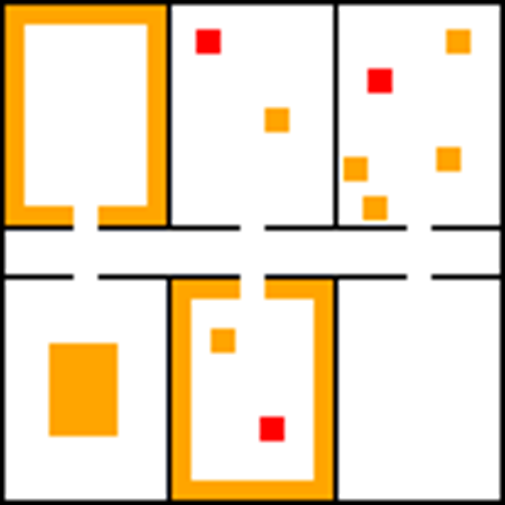
\includegraphics[width=0.5\hsize]{figures/Graph_Office.png}
  \caption{実験環境}
  \label{fig:env}
\end{figure}

\begin{figure}
  \centering
  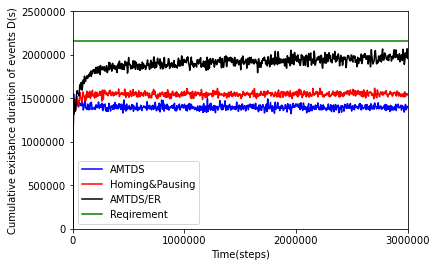
\includegraphics[width=0.8\hsize]{figures/ds_graph_3600_ave_ER_Office_600.png}
  \caption{$D(s)$の時間推移}
  \label{fig:ds_ER_Office}
  \centering
  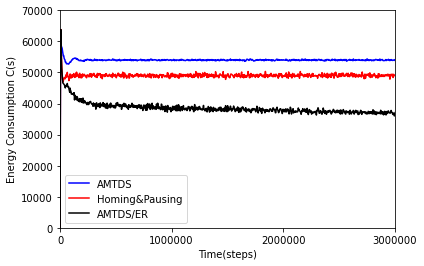
\includegraphics[width=0.8\hsize]{figures/cs_graph_3600_ave_ER_Office_600.png}
  \caption{$C(s)$の時間推移}
  \label{fig:cs_ER_Office}
\end{figure}

\section{実験}
\subsection{実験環境}
  実験環境は図\ref{fig:env}のような$101 \times 101$の2次元グリッド環境である.
  黒線は壁を表す.
  図\ref{fig:env}の色に従って,$p(v)$を次のように設定した.
  %
  \[
    p(v) = 
    \begin{cases}
      10^{-3}\ & \textrm{($v$が赤色の領域内の場合)}\\
      10^{-4}\ & \textrm{($v$がオレンジ色の領域内の場合)}\\
      10^{-6}\ & \textrm{($v$が白色の領域内の場合)}\\
    \end{cases}
  \]
  %
  エージェント数$|A|$は20体である.
  $D(s)$と$C(s)$の値は,独立した50回の試行による平均値である.

  \subsection{実験結果}
  従来手法であるAMTDSやAMTDS/ESCと,提案手法であるAMTDS/ERの$D(s)$と$C(s)$の時間推移を比較した結果を図\ref{fig:ds_ER_Office},\ref{fig:cs_ER_Office}に示す.
  なお,図\ref{fig:ds_ER_Office}内の緑色の直線が品質要求値である.
  これらの図より,AMTDS/ERは従来手法よりも,品質要求を満たしながら,より多くのエネルギー消費を削減できたことが分かる.

\section{結論}
本研究では,MACPPにおいて,各エージェントが学習したパラメータに基づいて,エネルギー節約行動を調整する手法を提案した.
実験の結果,提案手法は品質要求を満たしながら,より多くのエネルギー消費を削減できた.
今後は,エージェントが$p(v)$を学習しながらエネルギー消費量の削減を図る必要がある.

\bibliographystyle{junsrt}
\bibliography{ref}
\end{document}